\documentclass[11pt]{article}
\usepackage{mathblatt}
% gesetzt von werkzeuge/setzer.py (Sorte selbst) aus dem Lernweg L75
% und den Bankzeilen; Muster bau/proben/2026-10-09/hypotenuse-muster.
\usepackage{enumitem}
\usepackage{adjustbox,varwidth}
\newgeometry{a4paper,margin=18mm,top=15mm,bottom=20mm,footskip=9mm}
\pagestyle{fancy}\fancyhf{}\renewcommand{\headrulewidth}{0pt}
\fancyfoot[L]{\footnotesize\color{mbgrau}L75 \textperiodcentered{} Lösungen \textperiodcentered{} Körper erkennen, Netze, Schrägbilder}
\fancyfoot[R]{\footnotesize\color{mbgrau}\thepage}
\setlength{\parskip}{3pt}
\renewcommand{\kreuz}[1]{\mbox{$\square$\ #1}\quad}
\newcommand{\kreuzl}[1]{\par\hangindent1.4em\hangafter1\noindent$\square$\ #1}
\newcommand{\aufg}[3]{\par\noindent\makebox[0pt][r]{#3}\begin{minipage}[t]{\linewidth}#1\end{minipage}\par}
\newcommand{\aufgg}[4]{\par\noindent\makebox[0pt][r]{#4}\begin{minipage}[t]{0.6\linewidth}\vspace{0pt}#1\end{minipage}\hfill
  \begin{minipage}[t]{0.37\linewidth}\vspace{0pt}\centering #2\end{minipage}\par}
\newcommand{\nr}[1]{\makebox[7mm][l]{\textbf{#1}}}
\newcommand{\lsg}[3]{\par\noindent\begin{minipage}[t]{9mm}\textbf{#1}\end{minipage}%
  \begin{minipage}[t]{52mm}\raggedright\bfseries\boldmath #2\end{minipage}\hspace{3mm}%
  \begin{minipage}[t]{\dimexpr\linewidth-64mm\relax}\raggedright\small #3\end{minipage}\par\vspace{4pt}}
\newlength{\kr}
\makeatletter
\newcommand{\karomerk}[2]{\protected@write\@auxout{}{\string\karoseite{#1}{#2}{\thepage}}}
\newcommand{\karoseite}[3]{\expandafter\xdef\csname karo@#1@#2\endcsname{#3}}
\newcommand{\karohinweis}[3]{\karomerk{h}{#1}\ifcsname karo@k@#1\endcsname
  \ifnum\csname karo@k@#1\endcsname=0\csname karo@h@#1\endcsname\relax#2\else#3\fi
  \else#3\fi}
\makeatother
\begin{document}

\noindent{\Large\bfseries Lösungen}\hspace{1em}{\color{mbgrau}Körper erkennen, Netze, Schrägbilder}\par\smallskip
\noindent{\small Links das Ergebnis, rechts der Weg in kurzen Schritten. Stimmt dein Ergebnis nicht, such den ersten Schritt, der anders ist.}\par
\par\Needspace{25mm}\vspace{6pt}\noindent\colorbox{black!12}{\makebox[7mm]{\bfseries\strut A}}\hspace{2mm}{\bfseries Körper erkennen und zählen}\par\vspace{4pt}
\lsg{1.}{A Quader, B Zylinder, C Pyramide, D Kegel}{A Quader, B Zylinder, C Pyramide (quadratische Grundfläche), D Kegel}
\lsg{2.}{$5$ Ecken, $8$ Kanten, $5$ Flächen}{Ecken $= 4 + 1 = 5$; Kanten $= 4 + 4 = 8$; Flächen $= 1 + 4 = 5$}
\lsg{3.}{Sechseckprisma; $12$ Ecken, $18$ Kanten, $8$ Flächen}{Sechseckprisma; Ecken $= 6 + 6 = 12$; Kanten $= 6 + 6 + 6 = 18$; Flächen $= 2 + 6 = 8$}
\lsg{4.}{Nein: $2$ Stäbe fehlen, $1$ Kugel bleibt übrig}{Nein; Kanten $= 6 + 6 = 12$, es fehlen $12 - 10 = 2$ Stäbe; Ecken $= 6 + 1 = 7$, es bleibt $8 - 7 = 1$ Kugel übrig}
\par\Needspace{25mm}\vspace{6pt}\noindent\colorbox{black!12}{\makebox[7mm]{\bfseries\strut B}}\hspace{2mm}{\bfseries Würfelnetze: was liegt gegenüber?}\par\vspace{4pt}
\lsg{1.}{Q–S, R–T, P–U}{Q und S, R und T, P und U (senkrecht: R liegt dazwischen)}
\lsg{2.}{Nein: C hätte zwei Gegenflächen (A und E)}{Nein; in der Reihe liegt A gegenüber C und C gegenüber E – C hätte zwei Gegenflächen}
\lsg{3.}{$X = 4$, $Y = 5$, $Z = 1$}{$X = 4$ (gegenüber $3$), $Y = 5$ (gegenüber $2$), $Z = 1$ (gegenüber $6$)}
\lsg{4.}{Nein: $3$ und $5$ tauschen (oder $2$ und $4$)}{Nein; Paare $1 + 6 = 7$, $2 + 3 = 5$, $5 + 4 = 9$; $3$ und $5$ tauschen (oder $2$ und $4$)\par\smallskip \adjustbox{max width=\linewidth,max height=4cm}{\begin{varwidth}{50cm}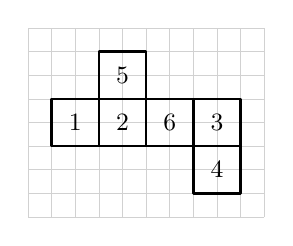
\begin{tikzpicture}[scale=0.6,font=\small,line join=round]\draw[black!18,line width=0.3pt,step=0.5] (-0.5,-0.5) grid (4.5,3.5);\draw[line width=0.9pt] (1,2) rectangle (2,3);\node at (1.5,2.5) {5};\draw[line width=0.9pt] (0,1) rectangle (1,2);\node at (0.5,1.5) {1};\draw[line width=0.9pt] (1,1) rectangle (2,2);\node at (1.5,1.5) {2};\draw[line width=0.9pt] (2,1) rectangle (3,2);\node at (2.5,1.5) {6};\draw[line width=0.9pt] (3,1) rectangle (4,2);\node at (3.5,1.5) {3};\draw[line width=0.9pt] (3,0) rectangle (4,1);\node at (3.5,0.5) {4};\end{tikzpicture}\end{varwidth}}}
\par\Needspace{25mm}\vspace{6pt}\noindent\colorbox{black!12}{\makebox[7mm]{\bfseries\strut C}}\hspace{2mm}{\bfseries Netze von Quader und anderen Körpern}\par\vspace{4pt}
\lsg{1.}{A Dreiecksprisma, B Pyramide, C Zylinder}{A Dreiecksprisma (zwei Dreiecke, drei Rechtecke), B Pyramide mit quadratischer Grundfläche (Quadrat, vier Dreiecke), C Zylinder (zwei Kreise, ein Rechteck)}
\lsg{2.}{$1$\,cm $\times$ $2$\,cm, rechts an „vorn“}{Es fehlt die zweite Seite: Breite $= 1$\,cm, Höhe $= 2$\,cm; rechts an „vorn“ (oder rechts an „hinten“)\par\smallskip \adjustbox{max width=\linewidth,max height=4cm}{\begin{varwidth}{50cm}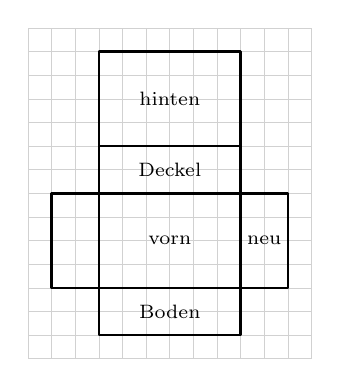
\begin{tikzpicture}[scale=0.6,font=\small,line join=round]\draw[black!18,line width=0.3pt,step=0.5] (-0.5,-0.5) grid (5.5,6.5);\draw[line width=0.9pt] (1,0) rectangle (4,1);\node[font=\scriptsize] at (2.5,0.5) {Boden};\draw[line width=0.9pt] (1,1) rectangle (4,3);\node[font=\scriptsize] at (2.5,2) {vorn};\draw[line width=0.9pt] (1,3) rectangle (4,4);\node[font=\scriptsize] at (2.5,3.5) {Deckel};\draw[line width=0.9pt] (1,4) rectangle (4,6);\node[font=\scriptsize] at (2.5,5) {hinten};\draw[line width=0.9pt] (0,1) rectangle (1,3);\draw[line width=0.9pt] (4,1) rectangle (5,3);\node[font=\scriptsize] at (4.5,2) {neu};\end{tikzpicture}\end{varwidth}}}
\lsg{3.}{Netz $6$\,cm $\times$ $4$\,cm (z.\,B. wie im Bild)}{Boden, Deckel, vorn und hinten je $4 \times 1$, Seiten $1 \times 1$ (in cm); Netz $6$\,cm breit, $4$\,cm hoch\par\smallskip \adjustbox{max width=\linewidth,max height=4cm}{\begin{varwidth}{50cm}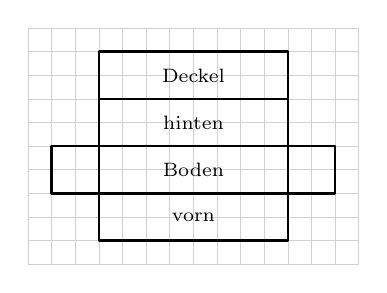
\begin{tikzpicture}[scale=0.6,font=\small,line join=round]\draw[black!18,line width=0.3pt,step=0.5] (-0.5,-0.5) grid (6.5,4.5);\draw[line width=0.9pt] (1,0) rectangle (5,1);\node[font=\scriptsize] at (3,0.5) {vorn};\draw[line width=0.9pt] (1,1) rectangle (5,2);\node[font=\scriptsize] at (3,1.5) {Boden};\draw[line width=0.9pt] (1,2) rectangle (5,3);\node[font=\scriptsize] at (3,2.5) {hinten};\draw[line width=0.9pt] (1,3) rectangle (5,4);\node[font=\scriptsize] at (3,3.5) {Deckel};\draw[line width=0.9pt] (0,1) rectangle (1,2);\draw[line width=0.9pt] (5,1) rectangle (6,2);\end{tikzpicture}\end{varwidth}}}
\lsg{4.}{Ja: Netz $10$\,cm $\times$ $12$\,cm}{Ja; das Netz ist $2 + 6 + 2 = 10$\,cm breit und $2 + 4 + 2 + 4 = 12$\,cm hoch, es passt auf $12$\,cm $\times$ $12$\,cm\par\smallskip \adjustbox{max width=\linewidth,max height=4cm}{\begin{varwidth}{50cm}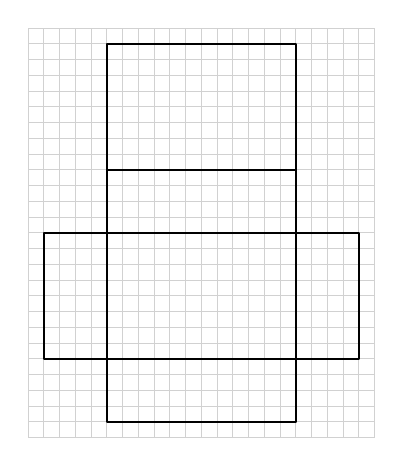
\begin{tikzpicture}[scale=0.4,font=\small,line join=round]\draw[black!18,line width=0.3pt,step=0.5] (-0.5,-0.5) grid (10.5,12.5);\draw[line width=0.9pt] (2,0) rectangle (8,2);\draw[line width=0.9pt] (2,2) rectangle (8,6);\draw[line width=0.9pt] (2,6) rectangle (8,8);\draw[line width=0.9pt] (2,8) rectangle (8,12);\draw[line width=0.9pt] (0,2) rectangle (2,6);\draw[line width=0.9pt] (8,2) rectangle (10,6);\end{tikzpicture}\end{varwidth}}}
\par\Needspace{25mm}\vspace{6pt}\noindent\colorbox{black!12}{\makebox[7mm]{\bfseries\strut D}}\hspace{2mm}{\bfseries Schrägbilder}\par\vspace{4pt}
\lsg{1.}{Schrägbild wie im Bild}{Vorderfläche $6 \times 6$ Kästchen; $3$ Kästchendiagonalen nach hinten; $3$ verdeckte Kanten gestrichelt\par\smallskip \adjustbox{max width=\linewidth,max height=4cm}{\begin{varwidth}{50cm}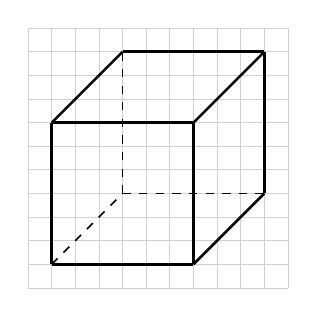
\begin{tikzpicture}[scale=0.6,font=\small,line join=round]\draw[black!18,line width=0.3pt,step=0.5] (-0.5,-0.5) grid (5,5);\draw[line width=0.9pt] (0,0) -- (3,0);\draw[line width=0.9pt] (3,0) -- (3,3);\draw[line width=0.9pt] (3,3) -- (0,3);\draw[line width=0.9pt] (0,0) -- (0,3);\draw[dashed,line width=0.6pt] (1.5,1.5) -- (4.5,1.5);\draw[line width=0.9pt] (4.5,1.5) -- (4.5,4.5);\draw[line width=0.9pt] (4.5,4.5) -- (1.5,4.5);\draw[dashed,line width=0.6pt] (1.5,1.5) -- (1.5,4.5);\draw[line width=0.9pt] (3,0) -- (4.5,1.5);\draw[dashed,line width=0.6pt] (0,0) -- (1.5,1.5);\draw[line width=0.9pt] (3,3) -- (4.5,4.5);\draw[line width=0.9pt] (0,3) -- (1.5,4.5);\end{tikzpicture}\end{varwidth}}}
\lsg{2.}{$4$\,cm lang, $2$\,cm hoch, $3$\,cm tief; $3$ verdeckt}{lang $8$ Kästchen $= 4$\,cm; hoch $4$ Kästchen $= 2$\,cm; tief $3$ Diagonalen $= 3$\,cm; verdeckt $3$ Kanten}
\lsg{3.}{Strecke $c$}{Sie geht von der Spitze senkrecht zur Mitte der Grundfläche; $a$ ist eine Kante, $b$ die Höhe einer Seitenfläche}
\lsg{4.}{$6$\,cm $\times$ $6$\,cm}{$4$ Diagonalen gehen $2$\,cm nach rechts und $2$\,cm hoch; Breite $4 + 2 = 6$\,cm, Höhe $4 + 2 = 6$\,cm\par\smallskip \adjustbox{max width=\linewidth,max height=4cm}{\begin{varwidth}{50cm}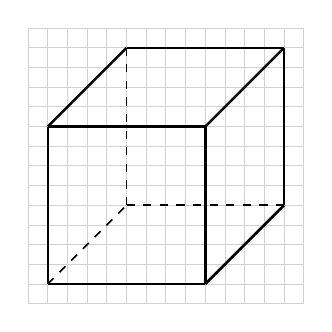
\begin{tikzpicture}[scale=0.5,font=\small,line join=round]\draw[black!18,line width=0.3pt,step=0.5] (-0.5,-0.5) grid (6.5,6.5);\draw[line width=0.9pt] (0,0) -- (4,0);\draw[line width=0.9pt] (4,0) -- (4,4);\draw[line width=0.9pt] (4,4) -- (0,4);\draw[line width=0.9pt] (0,0) -- (0,4);\draw[dashed,line width=0.6pt] (2,2) -- (6,2);\draw[line width=0.9pt] (6,2) -- (6,6);\draw[line width=0.9pt] (6,6) -- (2,6);\draw[dashed,line width=0.6pt] (2,2) -- (2,6);\draw[line width=0.9pt] (4,0) -- (6,2);\draw[dashed,line width=0.6pt] (0,0) -- (2,2);\draw[line width=0.9pt] (4,4) -- (6,6);\draw[line width=0.9pt] (0,4) -- (2,6);\end{tikzpicture}\end{varwidth}}}
\par\Needspace{25mm}\vspace{6pt}\noindent\colorbox{black!12}{\makebox[7mm]{\bfseries\strut T}}\hspace{2mm}{\bfseries Probetest}\par\vspace{4pt}
\lsg{1.}{$8$}{$4$ Kanten an der Grundfläche und $4$ zur Spitze}
\lsg{2.}{E}{in der Reihe C, D, E liegt genau D dazwischen; D grenzt an C}
\lsg{3.}{Pyramide mit dreieckiger Grundfläche}{vier Dreiecke, eines ist die Grundfläche, drei treffen sich in der Spitze}
\lsg{4.}{Schrägbild wie im Bild}{Vorderfläche $8 \times 4$ Kästchen; $1$ Kästchendiagonale nach hinten; $3$ verdeckte Kanten gestrichelt\par\smallskip \adjustbox{max width=\linewidth,max height=4cm}{\begin{varwidth}{50cm}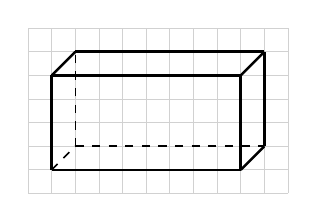
\begin{tikzpicture}[scale=0.6,font=\small,line join=round]\draw[black!18,line width=0.3pt,step=0.5] (-0.5,-0.5) grid (5,3);\draw[line width=0.9pt] (0,0) -- (4,0);\draw[line width=0.9pt] (4,0) -- (4,2);\draw[line width=0.9pt] (4,2) -- (0,2);\draw[line width=0.9pt] (0,0) -- (0,2);\draw[dashed,line width=0.6pt] (0.5,0.5) -- (4.5,0.5);\draw[line width=0.9pt] (4.5,0.5) -- (4.5,2.5);\draw[line width=0.9pt] (4.5,2.5) -- (0.5,2.5);\draw[dashed,line width=0.6pt] (0.5,0.5) -- (0.5,2.5);\draw[line width=0.9pt] (4,0) -- (4.5,0.5);\draw[dashed,line width=0.6pt] (0,0) -- (0.5,0.5);\draw[line width=0.9pt] (4,2) -- (4.5,2.5);\draw[line width=0.9pt] (0,2) -- (0.5,2.5);\end{tikzpicture}\end{varwidth}}}
\lsg{5.}{Ja: $96$\,cm nötig, $4$\,cm übrig}{Ja; ein Würfel hat $12$ Kanten: $12 \cdot 8 = 96$\,cm, es bleiben $100 - 96 = 4$\,cm übrig}
\end{document}
